
\begin{figure}
\begin{center}
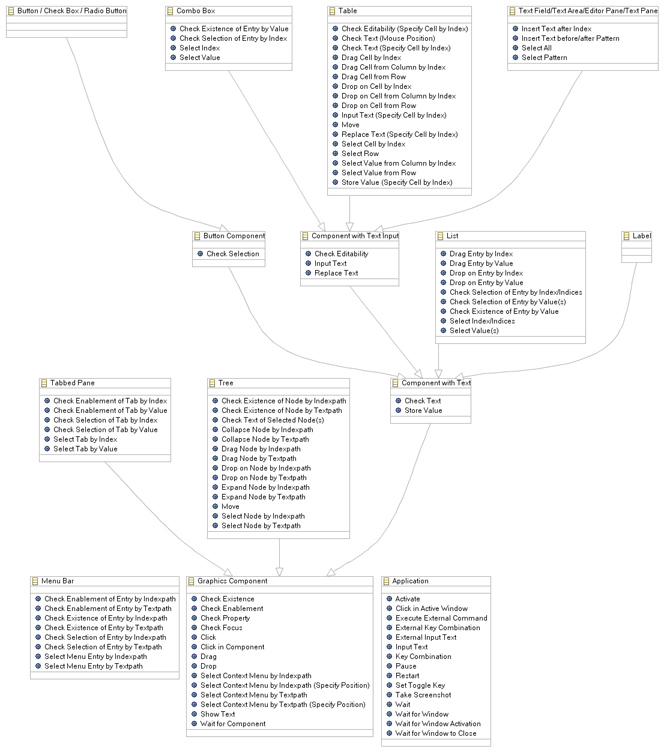
\includegraphics{Overview/PS/GUIdancerComponentHierarchysmall}
\caption{Component structure}
\label{comp}
\end{center}
\end{figure}

Figure \ref{comp} provides an overview of the concrete and abstract component structure. This figure can be interpreted as follows: the arrows show inheritance relations between the components. Thus, a \bxname{Label} component has no actions of its own, but inherits them all from \bxname{Component with Text}. The \bxname{Label} component also inherits any actions that \bxname{Component with Text} also inherited. In this case, these are the actions from \bxname{Graphics component}. 

\clearpage
